%\documentclass[a4paper,twoside,11pt]{report}
\documentclass[a4paper,singleside,11pt]{report}
\def\lingua{english}
% integration with pandoc new \tightlist control sequence
\def\tightlist{}
%\providecommand{\tightlist}{%
%  \setlength{\itemsep}{0pt}\setlength{\parskip}{0pt}}
\usepackage[T1]{fontenc}
\usepackage[utf8]{inputenc}
\DeclareUnicodeCharacter{20AC}{\euro{}}
\usepackage[official]{eurosym}
\usepackage{graphicx}
\usepackage{upquote}
\usepackage{epsfig}
\usepackage{ia_urb_thesis}
\usepackage[\lingua]{babel}
\usepackage{longtable}
\usepackage{booktabs}
%\usepackage{bibchapters}

\begin{document}

\titolo{Development, Testing, \\[5mm]
        and Continuous Integration \\[5mm]
        of Containerized Web Applications}
\candidato{Michele Sorcinelli}
\relatore{Chiar.mo Prof.~Alessandro Bogliolo}
\correlatori{Dott.~Luca Ferroni \\
             Dott.~Andrea Seraghiti \\
             Dott.~Lorenz Cuno Klopfenstein~}

\annoaccademico{2014-2015}


\copertinatesi 
\begin{tabular}{|p{.9\textwidth}|}
 \hline
 This work is licensed under a Creative Commons Attribution-ShareAlike 4.0
 License.
 \begin{center}
 \includegraphics[scale=1]{by-sa.eps}
 \end{center}
 © 2015 Michele Sorcinelli\\
 \hline
 \end{tabular}
\dedica{Ai miei genitori}
\indice
\indicefigure
\indicetabelle
\iniziatesto

\include{chapters/intro}
\include{chapters/context}
\include{chapters/ccba}
\include{chapters/e2e}
\include{chapters/ts}
\include{chapters/ci}
\include{chapters/conclusions}

\appendix
\include{chapters/appendix}
\begin{thebibliography}{999}

\bibitem{protractor}
\raggedright
{\em Protractor - end to end testing for AngularJS},
Available: https://angular.github.io/protractor/

\bibitem{gasistafelice}
\raggedright
beFair development team,
{\em Gasista Felice},
Available: https://befair.github.io/gasistafelice/

\bibitem{sharing-economy}
\raggedright
Benita Matofska, "What is the Sharing Economy?",
{\em The People Who Share},
Available: http://www.thepeoplewhoshare.com/blog/what-is-the-sharing-economy

\bibitem{docker-install}
Docker Inc. © 2015, "Supported Installation",
{\em Docker Documentation},
Available: https://docs.docker.com/installation/

\bibitem{docker-hub}
Docker Inc. © 2015,
{\em Docker Hub Registry - Repositories of Docker Images},
Available: https://hub.docker.com/

\bibitem{docker-compose}
\raggedright
Docker Inc. © 2015,
{\em Docker Compose},
Available: https://www.docker.com/docker-compose

\bibitem{docker-content-trust}
\raggedright
Docker Inc. © 2015,
{\em Introducing Docker Content Trust},
Available: https://blog.docker.com/2015/08/content-trust-docker-1-8/

\bibitem{docker-toolbox}
\raggedright
Docker Inc. © 2015,
{\em Docker Toolbox},
Available: https://www.docker.com/toolbox

\bibitem{xp-ci}
\raggedright
Don Wells © 1997-1999, All rights reserved, "Integrate Often",
{\em Extreme Programming},
Available: http://www.extremeprogramming.org/rules/integrateoften.html

\bibitem{unix}
\raggedright
Eric Steven Raymond © 2013, CC-BY-ND 1.0, "Chapter 1 - Philosophy",
{\em Basics of the Unix Philosophy},
Available: http://www.faqs.org/docs/artu/ch01s06.html

\bibitem{free-software}
\raggedright
Free Software Foundation Inc. © 2015, CC-BY-ND 4.0, "What is free software?"
{\em GNU Project - Free Software Foundation}
Available: https://www.gnu.org/philosophy/free-sw.html

\bibitem{node-to-iojs}
\raggedright
Galina Pankratova, InfoWorld Inc. © 1994-2015, All rights reserved, 4 December 2014,
{\em Why io.js decided to fork Node.js},
Available: http://www.infoworld.com/article/2855057/application-development/why-iojs-decided-to-fork-nodejs.html

\bibitem{two-way-binding}
\raggedright
Google Inc. © 2010-2015, CC-BY 3.0, "Step 4: Two-Way Data Binding",
{\em AngularJS Tutorial},
Available: https://docs.angularjs.org/tutorial/step\_04

\bibitem{ng-model}
\raggedright
Google Inc. © 2010-2015, CC-BY 3.0, "ngModel directive",
{\em AngularJS API Reference},
Available: https://docs.angularjs.org/api/ng/directive/ngModel

\bibitem{ng-bind}
\raggedright
Google Inc. © 2010-2015, CC-BY 3.0, "ngBind directive",
{\em AngularJS API Reference},
Available: https://docs.angularjs.org/api/ng/directive/ngBind

\bibitem{ng-repeat}
\raggedright
Google Inc. © 2010-2015, CC-BY 3.0, "ngRepeat directive",
{\em AngularJS API Reference},
Available: https://docs.angularjs.org/api/ng/directive/ngRepeat

\bibitem{agile-manifesto}
\raggedright
Kent Beck, Mike Beedle, Arie van Bennekum, Alistair Cockburn, Ward Cunningham,
Martin Fowler, James Grenning, Jim Highsmith, Andrew Hunt, Ron Jeffries, Jon
Kern, Brian Marick, Robert C. Martin, Steve Mellor, Ken Schwaber, Jeff
Sutherland, Dave Thomas, © 2001,
{\em Manifesto for Agile Software Development},
Available: http://www.agilemanifesto.org/

\bibitem{agile-principles}
\raggedright
Kent Beck, Mike Beedle, Arie van Bennekum, Alistair Cockburn, Ward Cunningham,
Martin Fowler, James Grenning, Jim Highsmith, Andrew Hunt, Ron Jeffries, Jon
Kern, Brian Marick, Robert C. Martin, Steve Mellor, Ken Schwaber, Jeff
Sutherland, Dave Thomas, © 2001,
{\em Principles behind the Agile Manifesto},
Available: http://www.agilemanifesto.org/principles.html

\bibitem{cloudflare-ecdsa}
\raggedright
Nick Sullivan, Cloudflare Inc. © 2015, 10 March 2014, "ECDSA vs RSA",
{\em ECDSA: The digital signature algorithm of a better internet},
Available: https://blog.cloudflare.com/ecdsa-the-digital-signature-algorithm-of-a-better-internet/

\bibitem{martinfowler-ci}
\raggedright
Martin Fowler ©, 01 May 2006,
{\em Continuous Integration},
Available: http://www.martinfowler.com/articles/continuousIntegration.html

\bibitem{martinfowler-ms}
\raggedright
Martin Fowler ©, 10 March 2014,
{\em Microservices},
Available: http://martinfowler.com/articles/microservices.html

\bibitem{devops}
\raggedright
Mike Loukides, O'Reilly Media, Inc. © 2015, June 7 2012
"What is DevOps?",
{\em the agile admin}.
Available: http://theagileadmin.com/what-is-devops/

\bibitem{mdn-map}
\raggedright
Mozilla Developer Network and individual Contributors © 2005-2015, CC-BY-SA 2.5, "Array.prototype.map()",
{\em Web Technology for developers},
Available: https://developer.mozilla.org/en-US/docs/Web/JavaScript/Reference/Global\_Objects/Array/map

\bibitem{wikipedia-docker}
\raggedright
Wikimedia Foundation Inc. and Contributors ©, CC-BY-SA 3.0,
last modified on 18 August 2012, "Docker (software)",
{\em Wikipedia, The Free Encyclopedia},
Available: https://en.wikipedia.org/wiki/Docker\_(software)

\end{thebibliography}


\ringraziamenti

First and foremost I would like to thank my parents, that supported me through
all my educational career, providing the necessary resources and encouragement.
Without their support, I would never been able to achieve these results. I would
like also to give my gratitude to Luca Ferroni, that provided a great support to
this work, welcomed me with open arms in his organization, and, most important,
he trusted in my ability even more than I did.

\end{document}
